\documentclass[conference]{IEEEtran}
\usepackage{amsmath,amssymb}
\usepackage{booktabs}
\usepackage{cite}
\usepackage{graphicx}
\usepackage{microtype}
\usepackage[caption=false,font=footnotesize]{subfig}
\usepackage{tikz}
\usetikzlibrary{arrows.meta,positioning,fit,calc}
\usepackage[hidelinks]{hyperref}
\usepackage{url}

\hypersetup{
  pdftitle={Native Binary-Weight Training Outperforms Zero-Shot Sign Projection in MNIST Diffusion},
  pdfauthor={Ayushman Bhattacharya, Anwesha Chakraborty, and Nihal Gazi},
  pdfkeywords={binary neural networks, diffusion models, quantization-aware training, post-training quantization, MNIST}
}

\newcommand{\dfid}{\ensuremath{\mathrm{dFID}}}
\newcommand{\dkid}{\ensuremath{\mathrm{dKID}}}
\begin{document}

\title{Native Binary-Weight Training Outperforms\\
Zero-Shot Sign Projection in MNIST Diffusion}

\author{
\IEEEauthorblockN{Ayushman Bhattacharya}
\IEEEauthorblockA{Pollinations AI\\ayushman.elixpo@gmail.com}
\and
\IEEEauthorblockN{Anwesha Chakraborty}
\IEEEauthorblockA{Dept. of CSE, JIS University\\anwesha.elixpo@gmail.com}
\and
\IEEEauthorblockN{Nihal Gazi}
\IEEEauthorblockA{Dept. of CSE (AI \& ML), IEM\\nihalg2006@gmail.com}
}

\maketitle

\begin{abstract}
Does severe failure after projecting a diffusion model to one-bit weights show
that its binary representation is unusable? We test that implication, rather
than propose a new quantizer, in a small MNIST residual U-Net. We compare
floating-point training, zero-shot per-channel sign/scale projection of a
trained model, binary-weight training from random initialization, floating-point
warm-started quantization-aware training (QAT), and a binary-weight/
binary-activation core. The primary FP32, native W1A32, and projected W1A32
comparison fixes the parameterization, data, training budget where applicable,
and 1,000-step ancestral sampler, with three independent training seeds. Native
W1A32 training obtains domain-feature Fr\'echet distance
$46.33\mathbin{\pm}17.24$, 28.4-fold lower than matched zero-shot projection
($1314.20\mathbin{\pm}314.96$), but remains substantially worse than FP32
($3.15\mathbin{\pm}0.38$). Warm QAT also recovers much of the projection loss, while
the W1A1 core retains a large distributional gap. An elementary feasible-set
argument explains why one projected floating-point solution is not an
impossibility certificate for the binary hypothesis class. The supported claim
is deliberately local: on MNIST, optimizing binary forwards reaches a much
better W1A32 solution than this zero-shot projection baseline; this does not
establish full W1A1 success, floating-point parity, or transfer to natural images.
\end{abstract}

\begin{IEEEkeywords}
binary neural networks, diffusion models, post-training quantization,
quantization-aware training, MNIST
\end{IEEEkeywords}

\section{Introduction}

Diffusion models repeatedly evaluate a time-conditioned denoiser, making model
memory and arithmetic attractive compression targets. Binary neural networks
replace many real-valued weights by signs and optional scales
\cite{hubara2016bnn,rastegari2016xnornet}. At the extreme, BiDM studies binary
weights and activations (W1A1) and motivates specialized architecture and
distillation by the severe degradation of naive full binarization
\cite{bidm2024}. BinaryDM studies accurate weight binarization at W1A4
\cite{binarydm2025}.

A narrower logical question precedes those system designs: if a trained FP32
denoiser collapses after sign projection, has the binary-weight representation
failed, or has a point optimized for a different forward model simply been
projected poorly? Our zero-shot post-training baseline evaluates only the
projected FP32 solution; it is not a calibrated PTQ method.
BinaryConnect-style training instead maintains latent real parameters while
using binary weights in every forward pass\cite{courbariaux2015binaryconnect}.
The two procedures need not reach the same binary point.

We isolate this distinction on MNIST. The primary precision conditions share
parameter names, shapes, U-Net graph, sampling procedure, and evaluation; all
trained stages use the same optimizer and 12-epoch budget. The experiment
supports three findings:
\begin{itemize}
  \item native W1A32 training reduces \dfid{} by 28.4-fold relative to matched
  zero-shot projection, so projection failure is not a certificate of binary-weight
  representational failure in this setting;
  \item warm-started QAT also recovers substantially, showing that random
  initialization is not uniquely necessary once binary forwards are optimized;
  and
  \item FP32 remains much better, while a W1A1 core remains weak; the result
  therefore neither contradicts the difficulty identified by BiDM nor
  establishes a general binary-diffusion solution.
\end{itemize}

The contribution is a controlled empirical distinction between projection and
optimization. The sign/scale quantizer, straight-through estimator (STE), and
residual components are standard and are not claimed as algorithmic novelty.

\section{Related Work}

Diffusion PTQ requires more care than applying an image-classification
quantizer unchanged. Q-Diffusion uses timestep-aware calibration and separate
treatment of shortcut activations\cite{li2023qdiffusion}; PTQD models and
corrects quantization noise accumulated through denoising
\cite{he2023ptqd}. These methods target multi-bit PTQ and are substantially more
sophisticated than our deliberately uncalibrated sign-projection baseline.
BinaryDM combines an evolvable binary basis with representation mimicking for
W1A4 diffusion\cite{binarydm2025}, whereas BiDM combines binary-specific
structure and distillation for W1A1 diffusion\cite{bidm2024}. We do not claim
competitive image quality or efficiency against these systems.

Binary-network research likewise shows that training procedure and activation
distributions matter. BinaryConnect optimizes latent real weights under binary
forwards\cite{courbariaux2015binaryconnect}; XNOR-Net introduces channel/filter
scaling\cite{rastegari2016xnornet}; Real-to-Binary Net uses a staged training
schedule\cite{martinez2020training}; and ReActNet learns activation shifts and
reshaping\cite{liu2020reactnet}. Our experiment uses only the standard
sign/scale and STE ingredients so that the intervention remains the training
path rather than a new binarizer.

\section{Projection and Constrained Optimization}

Let $\Theta_F$ be a floating-point parameter space, $\Theta_B$ the feasible
binary-weight space, $\mathcal L$ the diffusion training objective, and
$P:\Theta_F\rightarrow\Theta_B$ the baseline sign/scale projection. Let
$\theta_F^\star$ minimize $\mathcal L$ over $\Theta_F$ and
$\theta_B^\star$ minimize it over $\Theta_B$.

\paragraph{Feasible-set observation}
Assuming the minima exist, the loss of a projected floating-point optimum is an
upper bound on the optimal binary-constrained loss:
\begin{equation}
\mathcal L(\theta_B^\star)
\leq \mathcal L(P(\theta_F^\star)).
\end{equation}
Because $P(\theta_F^\star)\in\Theta_B$, it is one feasible point in the
minimization defining $\theta_B^\star$. Consequently, poor performance of
$P(\theta_F^\star)$ alone cannot establish that every member of $\Theta_B$
performs poorly. This is a direct consequence of the definition of a minimum,
not a new optimization theorem.

This elementary statement is not a convergence result. Native STE training is
not guaranteed to find $\theta_B^\star$, and diffusion quality is not determined
by training loss alone. It identifies exactly what the experiment must test:
whether optimization under binary forwards reaches a materially better feasible
point than zero-shot projection.

\begin{figure*}[t]
\centering
\resizebox{.98\textwidth}{!}{%
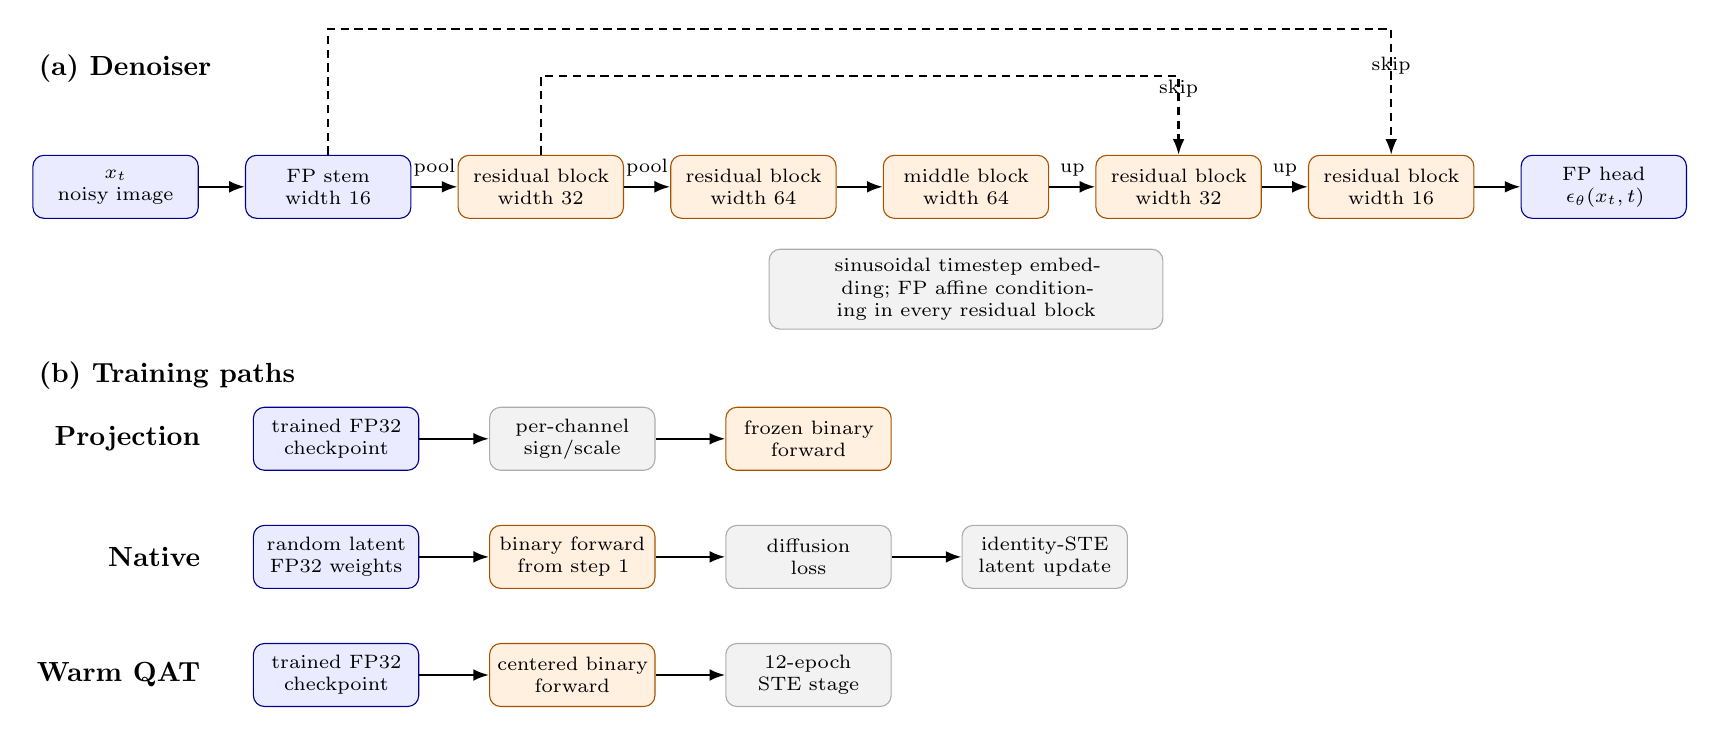
\begin{tikzpicture}[
  x=1mm,y=1mm,
  font=\scriptsize,
  box/.style={draw,rounded corners,minimum height=8mm,text width=19mm,
              align=center,inner xsep=1mm},
  fp/.style={box,fill=blue!8,draw=blue!55!black},
  bin/.style={box,fill=orange!12,draw=orange!65!black},
  op/.style={box,fill=gray!10,draw=gray!65},
  arrow/.style={-{Latex[length=2mm]},thick},
  skip/.style={-{Latex[length=2mm]},densely dashed,thick}
]
\node[fp] (xt) at (0,0) {$x_t$\\noisy image};
\node[fp] (stem) at (27,0) {FP stem\\width 16};
\node[bin] (e32) at (54,0) {residual block\\width 32};
\node[bin] (e64) at (81,0) {residual block\\width 64};
\node[bin] (mid) at (108,0) {middle block\\width 64};
\node[bin] (d32) at (135,0) {residual block\\width 32};
\node[bin] (d16) at (162,0) {residual block\\width 16};
\node[fp] (out) at (189,0) {FP head\\$\epsilon_\theta(x_t,t)$};
\draw[arrow] (xt)--(stem);
\draw[arrow] (stem)--node[above]{pool}(e32);
\draw[arrow] (e32)--node[above]{pool}(e64);
\draw[arrow] (e64)--(mid);
\draw[arrow] (mid)--node[above]{up}(d32);
\draw[arrow] (d32)--node[above]{up}(d16);
\draw[arrow] (d16)--(out);
\draw[skip] (stem.north) -- ++(0,16mm) -| node[pos=.72,above]{skip} (d16.north);
\draw[skip] (e32.north) -- ++(0,10mm) -| node[pos=.70,above]{skip} (d32.north);
\node[op,text width=48mm] at (108,-13) {sinusoidal timestep embedding; FP affine conditioning in every residual block};
\node[anchor=west,font=\bfseries] at (-11,15) {(a) Denoiser};

\node[anchor=east,font=\bfseries] at (12,-32) {Projection};
\node[fp] (ptq1) at (28,-32) {trained FP32\\checkpoint};
\node[op] (ptq2) at (58,-32) {per-channel\\sign/scale};
\node[bin] (ptq3) at (88,-32) {frozen binary\\forward};
\draw[arrow] (ptq1)--(ptq2); \draw[arrow] (ptq2)--(ptq3);

\node[anchor=east,font=\bfseries] at (12,-47) {Native};
\node[fp] (nat1) at (28,-47) {random latent\\FP32 weights};
\node[bin] (nat2) at (58,-47) {binary forward\\from step 1};
\node[op] (nat3) at (88,-47) {diffusion\\loss};
\node[op] (nat4) at (118,-47) {identity-STE\\latent update};
\draw[arrow] (nat1)--(nat2); \draw[arrow] (nat2)--(nat3); \draw[arrow] (nat3)--(nat4);

\node[anchor=east,font=\bfseries] at (12,-62) {Warm QAT};
\node[fp] (qat1) at (28,-62) {trained FP32\\checkpoint};
\node[bin] (qat2) at (58,-62) {centered binary\\forward};
\node[op] (qat3) at (88,-62) {12-epoch\\STE stage};
\draw[arrow] (qat1)--(qat2); \draw[arrow] (qat2)--(qat3);
\node[anchor=west,font=\bfseries] at (-11,-24) {(b) Training paths};
\end{tikzpicture}
}
\caption{Implementation-derived diagram. (a) Preactivation U-Net used by the
primary comparison; dashed routes are the actual stem-to-final-decoder and
32-channel encoder-to-first-decoder concatenative skips. Orange blocks use
W1A32 unless the W1A1 core is selected; normalization, conditioning, scales,
residual additions, and boundaries remain FP32. (b) Compared optimization
paths. The projection baseline performs no calibration or parameter updates.}
\label{fig:architecture}
\end{figure*}

\section{Controlled MNIST Experiment}

\subsection{Denoiser and binary forward}

For clean image $x_0$, noise $\epsilon$, and timestep $t$, every condition
minimizes the DDPM noise-prediction objective\cite{ho2020ddpm}:
\begin{equation}
\mathbb E_{x_0,t,\epsilon}\left\|\epsilon-\epsilon_\theta
\left(\sqrt{\bar\alpha_t}x_0+\sqrt{1-\bar\alpha_t}\epsilon,t\right)\right\|_2^2.
\end{equation}
The preactivation denoiser in Fig.~\ref{fig:architecture} is a residual U-Net
\cite{ronneberger2015unet} with base width 16, widths $[16,32,64]$, two
downsampling stages, two skip concatenations, GroupNorm, and sinusoidal time
embeddings\cite{wu2018groupnorm,vaswani2017attention}. It has 218,993 trainable
parameters.

For output filter $W_o$, the primary uncentered binary projection is
\begin{equation}
\widehat W_o=\alpha_o\operatorname{sign}(W_o),\qquad
\alpha_o=\operatorname{mean}(|W_o|).
\end{equation}
Latent FP32 parameters receive identity-STE gradients\cite{bengio2013ste}. The
centered ablation subtracts the filter mean before sign and scale. The W1A1 core
additionally signs block activations with a clipped-identity backward pass.
Input/output convolutions, normalization, time conditioning, biases, scales,
accumulation, and residual additions remain FP32; ``W1A1 core'' therefore does
not mean an end-to-end binary appliance.

\subsection{Conditions and optimization}

FP32 and native conditions train from random initialization for 12 epochs. The
zero-shot projection baseline loads the corresponding completed FP32 checkpoint,
changes only the convolutional forward weights, and performs neither calibration
nor optimization. Warm QAT loads that checkpoint and adds a full 12-epoch
binary-forward stage, for 24 total epochs. Native W1A32
crosses centered/uncentered projection with pre-/post-activation residual
ordering\cite{he2016preact}; the headline matched comparison is uncentered and
preactivation. Moving normalization for the postactivation ablation changes its
GroupNorm affine tensors, yielding 218,897 parameters rather than 218,993; it is
therefore an architectural ablation, not part of the exactly parameter-compatible
precision comparison.

We use the canonical 60,000/10,000 MNIST split\cite{lecun1998mnist}, scale
images to $[-1,1]$, and train with AdamW\cite{loshchilov2019adamw}, learning rate
$2\times10^{-4}$, weight decay $10^{-4}$, cosine decay, gradient clipping at 1,
batch size 256, and training seeds $\{0,1,2\}$. Sampling uses all 1,000 ancestral
DDPM steps. Each reported distribution contains 2,000 samples from a fixed
sampling seed independent of the training seed.

\subsection{Evaluation and controls}

An independently initialized MNIST classifier, trained only on the real training
split, reaches 98.03\% test accuracy and 1.44\% ten-bin expected calibration
error\cite{guo2017calibration}. Its penultimate features define domain-feature Fr\'echet distance
(\dfid)\cite{heusel2017fid}, unbiased polynomial-kernel distance
(\dkid)\cite{binkowski2018kid}, and $k=5$ density and coverage
\cite{naeem2020density}. We also report Jensen--Shannon divergence of predicted
class priors\cite{lin1991divergence}. These domain-specific values are not
comparable to ImageNet FID.
Finite-sample Fr\'echet estimates are biased\cite{chong2020unbiased}; with only
2,000 generated samples per seed, our \dfid{} values are descriptive effect-size
summaries rather than population estimates or significance tests.

A disjoint real--real split gives \dfid{} 0.076, density 0.969, and coverage
0.971. Clamped Gaussian noise gives \dfid{} 2278.24 and zero density/coverage.
Although that noise receives mean peak classifier confidence 1.000, confidence
is not used as a quality metric.

\section{Results}

\begin{table*}[t]
\centering
\caption{MNIST metrics, mean $\pm$ sample standard deviation over three training
seeds. Each seed contributes 2,000 samples from the same ancestral sampler.
Bold marks the best non-FP condition, not parity with FP32.}
\label{tab:results}
\small
\setlength{\tabcolsep}{4pt}
\begin{tabular}{lrrrrr}
\toprule
Condition & \dfid{} $\downarrow$ & \dkid{} $\downarrow$ & Density $\uparrow$ & Coverage $\uparrow$ & Class JS $\downarrow$ \\
\midrule
FP32 & $3.15\pm0.38$ & $0.056\pm0.013$ & $0.284\pm0.014$ & $0.195\pm0.017$ & $0.0329\pm0.0091$ \\
Native W1A32, uncentered/pre & $\mathbf{46.33\pm17.24}$ & $\mathbf{1.286\pm0.816}$ & $\mathbf{0.022\pm0.005}$ & $\mathbf{0.033\pm0.010}$ & $\mathbf{0.2946\pm0.0202}$ \\
Warm QAT W1A32, centered/pre & $66.45\pm28.49$ & $4.945\pm3.686$ & $0.019\pm0.004$ & $0.032\pm0.004$ & $0.3196\pm0.0593$ \\
Native W1A1 core & $204.55\pm69.77$ & $41.03\pm25.01$ & $0.005\pm0.002$ & $0.009\pm0.004$ & $0.3395\pm0.0268$ \\
Projected W1A32, centered/pre & $871.12\pm717.34$ & $1581.31\pm2433.16$ & $0$ & $0$ & $0.5326\pm0.0002$ \\
Projected W1A32, unc./pre & $1314.20\pm314.96$ & $2467.50\pm1549.51$ & $0$ & $0$ & $0.5314\pm0.0023$ \\
\bottomrule
\end{tabular}
\end{table*}

\paragraph{Native optimization outperforms zero-shot projection}
Table~\ref{tab:results} gives the main comparison. Native W1A32 has 28.4-fold
lower mean \dfid{} than its matched projection configuration and nonzero density and
coverage. This is an empirical witness that a binary-forward optimization path
can reach a substantially better model than sign-projecting the FP32 endpoint.
It does not show that all binary training succeeds: the standard deviation is
large and every reported distribution metric remains worse than FP32.

\paragraph{Warm QAT also recovers}
Warm QAT obtains \dfid{} $66.45\pm28.49$, 13.1-fold below the mean of its
matched centered projection baseline ($871.12\pm717.34$). The projected
baseline is highly variable, and warm QAT uses an additional 12-epoch stage, so
this ratio is descriptive rather than a sample-efficiency claim. Its centered
configuration is not a strictly matched comparison to the best uncentered native
row. Native training is superior to zero-shot projection, not necessarily to
every warm-start or teacher-dependent procedure.

\paragraph{W1A1 remains difficult}
The W1A1 core improves over both zero-shot W1A32 projections in \dfid{} but has density 0.005
and coverage 0.009. Our experiment therefore does not refute BiDM's observation
that simultaneous weight and activation binarization is difficult. It instead
isolates a weaker but useful statement about one-bit weights with FP32
activations.

\begin{figure}[t]
\centering
\subfloat[FP32]{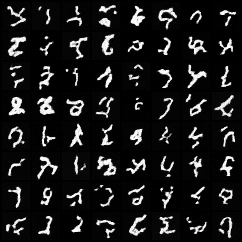
\includegraphics[width=.31\columnwidth]{figures/results/mnist-fp.png}}\hfill
\subfloat[Native W1A32]{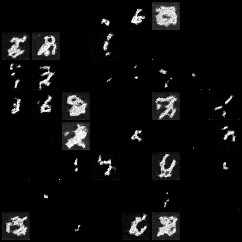
\includegraphics[width=.31\columnwidth]{figures/results/mnist-native-w1a32.png}}\hfill
\subfloat[Projected W1A32]{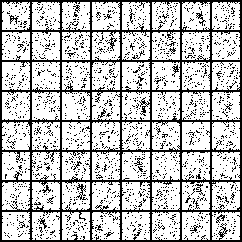
\includegraphics[width=.31\columnwidth]{figures/results/mnist-ptq-w1a32.png}}
\caption{Training seed 0 and sampling seed 4242. Native binary-weight training
retains digit-like structure but remains visibly below FP32; zero-shot sign
projection produces non-digit structure.}
\label{fig:samples}
\end{figure}

\begin{table}[t]
\centering
\caption{Native W1A32 architectural ablation (mean \dfid{}; lower is better).}
\label{tab:ablation}
\small
\begin{tabular}{lrr}
\toprule
Residual order & Uncentered & Centered \\
\midrule
Pre-activation & $46.33$ & $99.50$ \\
Post-activation & $84.26$ & $82.46$ \\
\bottomrule
\end{tabular}
\end{table}

\paragraph{Architecture does not yield a universal rule}
Table~\ref{tab:ablation} shows an interaction: preactivation helps only without
centering. Centering also raises mean latent-to-projected angular error from
$33.29^\circ$ to $34.05^\circ$ in that pair. Neither choice is therefore a
universal safeguard against degradation.

\section{Scope, Limitations, and Reproducibility}

This is an MNIST existence result for a small unconditional model. Three seeds
expose high variance but are insufficient for fine-grained significance claims;
2,000 samples per seed make absolute metric estimates noisier than common
50,000-sample evaluations. A separate compact CIFAR-10 attempt is intentionally
excluded from the evidence because its FP32 control also failed, so it could not
adjudicate binary versus floating-point quality on natural images. No theorem
here establishes STE convergence, score approximation, or scaling behavior.

Binary convolutions contain 195,328 of 218,993 parameters. Counting one bit per
binary weight plus FP32 per-output-channel scales and all remaining FP32 tensors
gives a calculated raw payload of 121,316 bytes versus 875,972 bytes for FP32, a
7.22$\times$ reduction. This excludes container and runtime overhead and is not
a hardware measurement: ordinary framework convolutions still execute
floating-point operations, and we claim no latency or energy improvement.

The released pipeline\cite{monodiffuseRepo} records configurations, seeds,
environment versions, the exact experiment commit, checkpoint SHA-256 values,
histories, metrics, controls, and a packed export. The repository README maps
the exact experiment entry points and MNIST artifact directories. Tests cover
parameter compatibility, forward shapes, diffusion schedules, metric controls,
and physical packing.

\section{Conclusion}

Zero-shot sign projection answers whether one particular FP32 endpoint survives
binarization; it does not answer whether binary-forward optimization can find a
better binary-weight solution. In a controlled MNIST diffusion model, native
W1A32 training reduces domain-feature distance by 28.4-fold relative to matched
projection, while warm QAT also recovers substantially. The result is meaningful but
bounded: FP32 remains much better, W1A1 remains weak, and natural-image transfer
is unresolved. Future binary-diffusion comparisons should distinguish native,
warm-started, distilled, and zero-shot training paths rather than treating
zero-shot projection failure as the limit of the representation.

\smallskip\noindent\textbf{Code availability.}
Source, checkpoints, packed weights, and evaluation artifacts are available at
\url{https://github.com/elixpo/monodiffuse}.

\IEEEtriggeratref{11}
\bibliographystyle{IEEEtran}
\bibliography{references}
\end{document}
